%-----------------------------------------------------------------------------------------
% Autor dieser Vorlage:
% Yllonier (https://github.com/YlloNieR)
% Lizenz: Creative Commons 4.0 Namensnennung
% -----------------------------------------------------------------------------------------

\documentclass[fontsize=11pt,paper=a4,oneside,svgnames,table]{scrreprt}
% Ausgangs Schriftgröße 11pt
% Papierformat A4 Format
% oneside 1:1 Verhältnis
% svgnames für Namen wie z.B. "AliceBlue"
% table für Tabellen Verwendung

\renewcommand*{\chapterheadstartvskip}{\vspace*{.5\baselineskip}}
%\vspace*{2.3\baselineskip} = ORIGINAL
% Abstand einstellen

%!TEX root = rootOfProject.tex
\usepackage[utf8]{inputenc} 
% encoding für Umlaute
\usepackage[ngerman]{babel}
% ermöglicht deutsche Silbentrennung
\usepackage[T1]{fontenc} 
% Fontencoding Format ermöglicht Suche nach Worten mit Ö
\usepackage{graphicx} 
% um Grafiken mit einzubinden z.B. jpeg
\usepackage{lmodern}
% mehr Schriftarten
\usepackage{geometry}
% für Layout config
\usepackage[toc,section=section,acronym]{glossaries}
% erstellt Glossar 
\usepackage{silence}
\WarningFilter{scrreprt}{Usage of package `fancyhdr'}
% verhindert von fancyhdr Error
\usepackage{pdfpages}
% Zur Einbindung externer pdf Dateien
\usepackage[printonlyused]{acronym}
% Zur Verwenung von Acronymen / Abkürzungen
\usepackage{fancyhdr}
% Für Header und Footer Style

% \usepackage{helvet}
% Schriftart= helvetica 
% \renewcommand{\familydefault}{\sfdefault}

\usepackage{uarial}
% Schriftart= arial
\renewcommand{\familydefault}{\sfdefault}
% setze default Schriftart
\usepackage{ragged2e}
% Schriftarten wie Blockschrift

\usepackage{xcolor}
% Für Tabellenfarben wie Projektphasen

\usepackage[%
backend=biber
,citestyle=numeric-comp
,sorting=none
,sortcites=true
,block=none
]{biblatex}
\addbibresource{bibShow.bib}




%!TEX root = rootOfProject.tex
% verwendete Variabeln:
\newcommand{\auditCommittee}{IHK Stadtname}

\newcommand{\mainTitle}{Dokumentation zur betrieblichen Projektarbeit}
\newcommand{\projectTitleLong}{ProjektarbeitnameLang}
\newcommand{\projectTitleShort}{ProjektarbeitnameKurz}

\newcommand{\companyNameLong}{FirmennameLang}
\newcommand{\companyNameShort}{FirmennameKurz}

\newcommand{\companyLocationStreet}{Strasse}
\newcommand{\companyLocationNumber}{Nummer}
\newcommand{\companyLocationPostcode}{PLZ}
\newcommand{\companyLocationCity}{Stadt}
\newcommand{\companyLocationState}{Bundesland}

\newcommand{\apprenticeship}{Fachinformatiker für ...}
\newcommand{\deliveryPlace}{IhkOrt}
\newcommand{\submissionDate}{20.09.2021}
\newcommand{\authorName}{Yllonier}
\newcommand{\projectManager}{Vorname Nachname}
\newcommand{\dateOfCreation}{12.08.2021}
\newcommand{\logo}{img/sample-logo.png}

% in Metadaten verwendete Variabeln
\title{\mainTitle}
\author{\authorName}




\pagenumbering{arabic}
%!TEX root = rootOfProject.tex
\makeglossaries
\newglossaryentry{imcp}
{
	name=ICMP,
	description={
		Das Internet Control Message Protocol (ICMP) dient in Rechnernetzwerken dem Austausch von Informations- und Fehlermeldungen über das Internet-Protokoll in der Version 4 (IPv4). Für IPv6 existiert ein ähnliches Protokoll mit dem Namen ICMPv6. ... ICMP-Nachrichten werden in IP-Paketen gekapselt.
	}
}
\newglossaryentry{latex}
{
	name=latex,
	description={
		Is a markup language specially suited 
		for scientific documents}
}

\newglossaryentry{ip}
{
	name=ip,
	description={
		Das Internet Protocol (IP) ist ein in Computernetzen weit verbreitetes Netzwerkprotokoll und stellt durch seine Funktion die Grundlage des Internets dar. Das IP ist die Implementierung der Internetschicht des TCP/IP-Modells bzw. der Vermittlungsschicht (engl. Network Layer) des OSI-Modells.
	}
}
%!TEX root = rootOfProject.tex

\fancypagestyle{plain}{
	\fancyhf{}% clear all fields
	\renewcommand{\headrulewidth}{0.4pt} %obere Trennlinie Dicke
	\fancyhead[L]{\projectTitleShort}
	\fancyhead[C]{\nouppercase{\leftmark}}
	\fancyhead[R]{\companyNameShort 
\includegraphics[scale=0.02]{img/sample-logo.png}}%
	\renewcommand{\footrulewidth}{0.4pt} %untere Trennlinie Dicke
	\fancyfoot[L]{\authorName}
	\fancyfoot[C]{\rightmark}
	\fancyfoot[R]{\thepage}%
}
% style für alle ersten Seiten
\pagestyle{fancy}
\renewcommand{\headrulewidth}{0.4pt} %obere Trennlinie Dicke
\lhead{\projectTitleShort}
\chead{\nouppercase{\leftmark}}
\rhead{\companyNameShort 
\includegraphics[scale=0.02]{img/sample-logo.png}}
\lfoot{\authorName}
\cfoot{}
\rfoot{\thepage}
\renewcommand{\footrulewidth}{0.4pt} %untere Trennlinie Dicke
% style für alle zusätzlichen Seiten

\fancypagestyle{attachmentStyle}{
	\fancyhf{}% clear all fields
	\renewcommand{\headrulewidth}{0.4pt} %obere Trennlinie Dicke
	\fancyhead[L]{\projectTitleShort}
	\fancyhead[R]{\companyNameShort 
\includegraphics[scale=0.02]{img/sample-logo.png}}%	
	\renewcommand{\footrulewidth}{0.4pt} %untere Trennlinie Dicke
	\fancyfoot[L]{\authorName}
	\fancyfoot[R]{\thepage}%	
}	



\begin{document}
	%!TEX root = ../rootOfProject.tex
\begin{titlepage}	
\centering	
{\LARGE \auditCommittee \par}
\vspace{1cm}
{\Large \mainTitle \par}
\vspace{1.5cm}
{\huge\bfseries \projectTitleLong \par}
\vspace{1cm}
{\Large\itshape \authorName \par}
\vspace{1cm}
{\Large\bfseries \apprenticeship \par}
\vspace{1cm}
{\Large\itshape \companyNameLong (\companyNameShort) \par}
\vspace{1cm}
{\large\itshape \companyLocationStreet \companyLocationNumber, \companyLocationPostcode \companyLocationCity, \companyLocationState \par}

\vfill
unter der Aufsicht von \par
Projektverantwortlicher \projectManager \par
**  Telefonnummer
\vfill		
% Footer
{\large \dateOfCreation \par}
\vspace{1cm}
\small 
Diese Arbeit wurde in \LaTeX  geschrieben und mit TeXworks kompiliert. \\ % nächste Zeile
\small
\noindent
\begin{justify}
	Dieses Werk einschließlich seiner Teile ist \textbf{urheberrechtlich geschützt}.
	Jede Verwertung außerhalb der engen Grenzen des Urheberrechtgesetzes ist ohne
	Zustimmung des Autors unzulässig und strafbar. Das gilt insbesondere für
	Vervielfältigungen, Übersetzungen, Mikroverfilmungen sowie die Einspeicherung
	und Verarbeitung in elektronischen Systemen.
\end{justify}

\end{titlepage}
	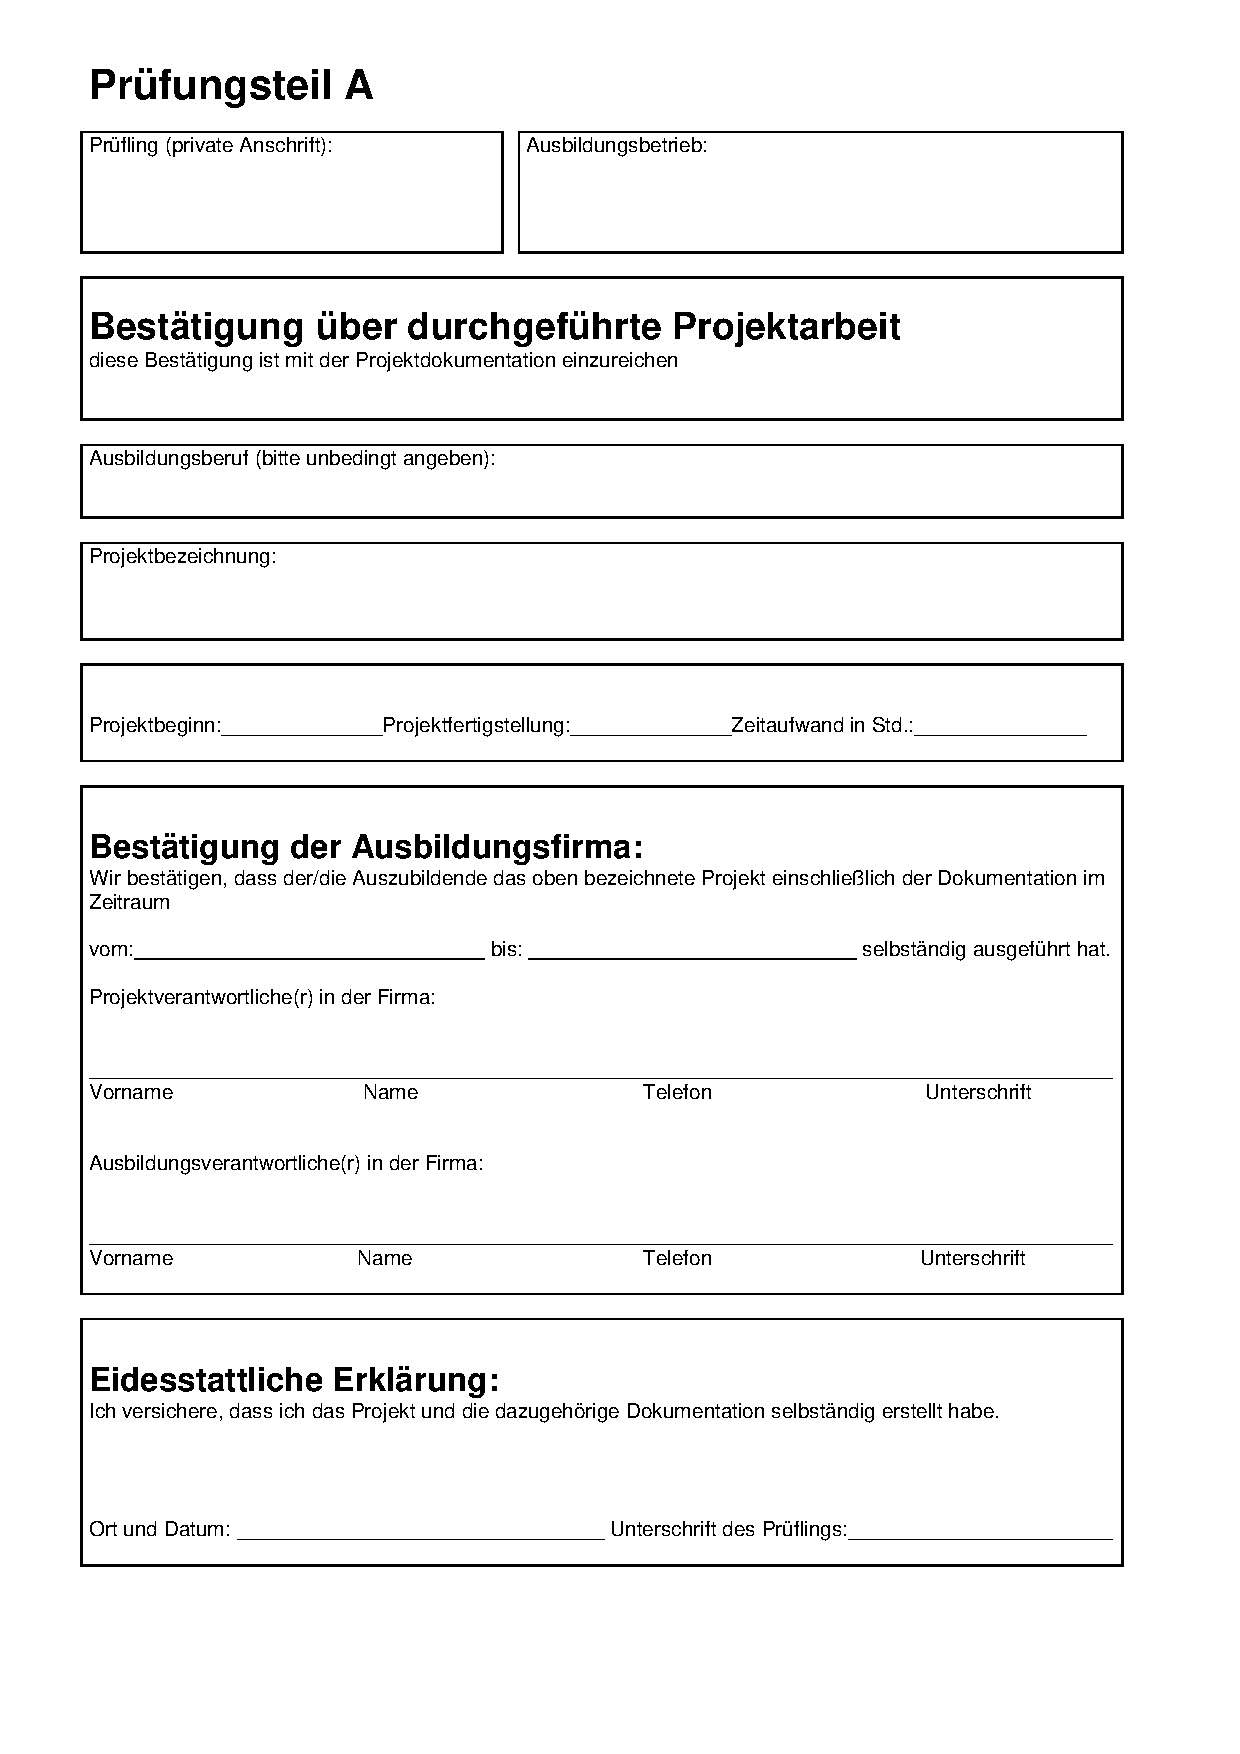
\includepdf{img/DeckblattIHK.pdf}
	%!TEX root = ../rootOfProject.tex
\clearpage
\addsec{Eidesstattliche Erklärung}
Ich, \authorName, versichere hiermit, dass ich meine \textbf{\projectTitleShort} mit dem
Thema
\begin{quote}
	\textit{\projectTitleLong}
\end{quote}
selbständig verfasst und keine anderen als die angegebenen Quellen und Hilfsmittel benutzt habe,
wobei ich alle wörtlichen und sinngemäßen Zitate als solche gekennzeichnet habe. Die Arbeit
wurde bisher keiner anderen Prüfungsbehörde vorgelegt und auch nicht veröffentlicht.\par\bigskip
% behebt overfull 10000 Bug

\deliveryPlace, den \submissionDate\par
\rule[-0.1cm]{5.5cm}{0.5pt}\par
\authorName
	
	%!TEX root = rootOfProject.tex
\newgeometry{
left=3.3cm,
top=2.1cm,
right=3cm,
bottom=3cm,
includeheadfoot
}

\setlength{\baselineskip}{16.5pt}
% Zeilenabstand 1.5fach = 1.5 * Fontsize = lineheight | \baselineskip

	{      
		\fancypagestyle{plain}         % Re-definition removes numbers from first page.
		{
			\fancyhf{}% clear all fields
			\renewcommand{\headrulewidth}{0.4pt} %obere Trennlinie Dicke
			\fancyhead[L]{\projectTitleShort}
			\fancyhead[R]{\companyNameShort 
\includegraphics[scale=0.02]{img/sample-logo.png}}%	
			\renewcommand{\footrulewidth}{0.4pt} %untere Trennlinie Dicke
			\fancyfoot[L]{\authorName}
			\fancyfoot[R]{\thepage}%
		}
		\tableofcontents	
		% Inhaltsverzeichnis
		\thispagestyle{attachmentStyle}
	}

	\thispagestyle{plain}
	%!TEX root =  ../rootOfProject.tex
\chapter[Einleitung]{Einführung in die Informatik}
\label{cha:Einleitung}
\section{Praktikumsbetrieb}
\label{sec:Praktikumsbetrieb}
Lorem ipsum dolor sit amet, consetetur sadipscing elitr, sed diam nonumy eirmod tempor invidunt ut labore et dolore magna aliquyam erat, sed diam voluptua. At vero eos et accusam et justo duo dolores et ea rebum. Stet clita kasd gubergren, no sea takimata sanctus est Lorem ipsum dolor sit amet. Lorem ipsum dolor sit amet, consetetur sadipscing elitr, sed diam nonumy eirmod tempor invidunt ut labore et dolore magna aliquyam erat, sed diam voluptua. At vero eos et accusam et justo duo dolores et ea rebum. Stet clita kasd gubergren, no sea takimata sanctus est Lorem ipsum dolor sit amet.

\section{Projektumfeld}
Lorem ipsum dolor sit amet, consetetur sadipscing elitr, sed diam nonumy eirmod tempor invidunt ut labore et dolore magna aliquyam erat, sed diam voluptua. At vero eos et accusam et justo duo dolores et ea rebum. Stet clita kasd gubergren, no sea takimata sanctus est Lorem ipsum dolor sit amet. Lorem ipsum dolor sit amet, consetetur sadipscing elitr, sed diam nonumy eirmod tempor invidunt ut labore et dolore magna aliquyam erat, sed diam voluptua. At vero eos et accusam et justo duo dolores et ea rebum. Stet clita kasd gubergren, no sea takimata sanctus est Lorem ipsum dolor sit amet.
\subsection{Zielsetzung}
\label{sub:Zielsetzung}
Lorem ipsum dolor sit amet, consetetur sadipscing elitr, sed diam nonumy eirmod tempor invidunt ut labore et dolore magna aliquyam erat, sed diam voluptua. At vero eos et accusam et justo duo dolores et ea rebum. Stet clita kasd gubergren, no sea takimata sanctus est Lorem ipsum dolor sit amet. Lorem ipsum dolor sit amet, consetetur sadipscing elitr, sed diam nonumy eirmod tempor invidunt ut labore et dolore magna aliquyam erat, sed diam voluptua. At vero eos et accusam et justo duo dolores et ea rebum. Stet clita kasd gubergren, no sea takimata sanctus est Lorem ipsum dolor sit amet.
\section{Abschluss}
\ref{sub:Zielsetzung} 
Lorem ipsum dolor sit amet, consetetur sadipscing elitr, sed diam nonumy eirmod tempor invidunt ut labore et dolore magna aliquyam erat, sed diam voluptua. At vero eos et accusam et justo duo dolores et ea rebum. Stet clita kasd gubergren, no sea takimata sanctus est Lorem ipsum dolor sit amet. Lorem ipsum dolor sit amet, consetetur sadipscing elitr, sed diam nonumy eirmod tempor invidunt ut labore et dolore magna aliquyam erat, sed diam voluptua. At vero eos et accusam et justo duo dolores et ea rebum. Stet clita kasd gubergren, no sea takimata sanctus est Lorem ipsum dolor sit amet.

	%!TEX root =  ../rootOfProject.tex

\chapter{Projektplanung}
\section{Zeitlicher Projektplan}
Lorem ipsum dolor sit amet, consectetuer adipiscing elit. Ut purus elit,
vestibulum ut, placerat ac, adipiscing vitae, felis. Curabitur dictum gravida
mauris. Nam arcu libero, nonummy eget, consectetuer id, vulputate a, magna.
Donec vehicula augue eu neque. Pellentesque habitant morbi tristique senectus
et netus et malesuada fames ac turpis egestas. Mauris ut leo. Cras viverra
metus rhoncus sem. Nulla et lectus vestibulum urna fringilla ultrices. Phasellus
eu tellus sit amet tortor gravida placerat. Integer sapien est, iaculis in, pretium
quis, viverra ac, nunc. Praesent eget sem vel leo ultrices bibendum. Aenean
faucibus. Morbi dolor nulla, malesuada eu, pulvinar at, mollis ac, nulla. Cur-
abitur auctor semper nulla. Donec varius orci eget risus. Duis nibh mi, congue
eu, accumsan eleifend, sagittis quis, diam. Duis eget orci sit amet orci dignissim
rutrum.
\section{Ist-Analyse}
Lorem ipsum dolor sit amet, consetetur sadipscing elitr, sed diam nonumy eirmod tempor invidunt ut labore et dolore magna aliquyam erat, sed diam voluptua. At vero eos et accusam et justo duo dolores et ea rebum. Stet clita kasd gubergren, no sea takimata sanctus est Lorem ipsum dolor sit amet. Lorem ipsum dolor sit amet, consetetur sadipscing elitr, sed diam nonumy eirmod tempor invidunt ut labore et dolore magna aliquyam erat, sed diam voluptua. At vero eos et accusam et justo duo dolores et ea rebum. Stet clita kasd gubergren, no sea takimata sanctus est Lorem ipsum dolor sit amet.
\section{Soll-Analyse}
Lorem ipsum dolor sit amet, consetetur sadipscing elitr, sed diam nonumy eirmod tempor invidunt ut labore et dolore magna aliquyam erat, sed diam voluptua. At vero eos et accusam et justo duo dolores et ea rebum. Stet clita kasd gubergren, no sea takimata sanctus est Lorem ipsum dolor sit amet. Lorem ipsum dolor sit amet, consetetur sadipscing elitr, sed diam nonumy eirmod tempor invidunt ut labore et dolore magna aliquyam erat, sed diam voluptua. At vero eos et accusam et justo duo dolores et ea rebum. Stet clita kasd gubergren, no sea takimata sanctus est Lorem ipsum dolor sit amet.
\section{Ressourcenplanung}
Lorem ipsum dolor sit amet, consetetur sadipscing elitr, sed diam nonumy eirmod tempor invidunt ut labore et dolore magna aliquyam erat, sed diam voluptua. At vero eos et accusam et justo duo dolores et ea rebum. Stet clita kasd gubergren, no sea takimata sanctus est Lorem ipsum dolor sit amet. Lorem ipsum dolor sit amet, consetetur sadipscing elitr, sed diam nonumy eirmod tempor invidunt ut labore et dolore magna aliquyam erat, sed diam voluptua. At vero eos et accusam et justo duo dolores et ea rebum. Stet clita kasd gubergren, no sea takimata sanctus est Lorem ipsum dolor sit amet.
\subsection{Recherche Software und Hardware Komponenten}
Lorem ipsum dolor sit amet, consetetur sadipscing elitr, sed diam nonumy eirmod tempor invidunt ut labore et dolore magna aliquyam erat, sed diam voluptua. At vero eos et accusam et justo duo dolores et ea rebum. Stet clita kasd gubergren, no sea takimata sanctus est Lorem ipsum dolor sit amet. Lorem ipsum dolor sit amet, consetetur sadipscing elitr, sed diam nonumy eirmod tempor invidunt ut labore et dolore magna aliquyam erat, sed diam voluptua. At vero eos et accusam et justo duo dolores et ea rebum. Stet clita kasd gubergren, no sea takimata sanctus est Lorem ipsum dolor sit amet.
\subsection{Angebotseinholung und Vergleich}
Lorem ipsum dolor sit amet, consetetur sadipscing elitr, sed diam nonumy eirmod tempor invidunt ut labore et dolore magna aliquyam erat, sed diam voluptua. At vero eos et accusam et justo duo dolores et ea rebum. Stet clita kasd gubergren, no sea takimata sanctus est Lorem ipsum dolor sit amet. Lorem ipsum dolor sit amet, consetetur sadipscing elitr, sed diam nonumy eirmod tempor invidunt ut labore et dolore magna aliquyam erat, sed diam voluptua. At vero eos et accusam et justo duo dolores et ea rebum. Stet clita kasd gubergren, no sea takimata sanctus est Lorem ipsum dolor sit amet.
\subsection{Entscheidung in Absprache mit der Geschäftsführung}
Lorem ipsum dolor sit amet, consetetur sadipscing elitr, sed diam nonumy eirmod tempor invidunt ut labore et dolore magna aliquyam erat, sed diam voluptua. At vero eos et accusam et justo duo dolores et ea rebum. Stet clita kasd gubergren, no sea takimata sanctus est Lorem ipsum dolor sit amet. Lorem ipsum dolor sit amet, consetetur sadipscing elitr, sed diam nonumy eirmod tempor invidunt ut labore et dolore magna aliquyam erat, sed diam voluptua. At vero eos et accusam et justo duo dolores et ea rebum. Stet clita kasd gubergren, no sea takimata sanctus est Lorem ipsum dolor sit amet.
\subsection{Gesamtkostenaufstellung}

\begin{table}[]
	\centering
	\begin{tabular}{|l|c|}
		\hline
		\rowcolor[HTML]{A3C7DB} 
		\multicolumn{1}{|c|}{\cellcolor[HTML]{A3C7DB}\textbf{Projektphase}} & \textbf{geplante Zeit} \\ \hline
		Analysephase                                                        & 2 h                    \\ \hline
		Entwurfsphase                                                       & 4 h                    \\ \hline
		Integrationsphase                                                   & 5 h                    \\ \hline
	\end{tabular}
    \label{tab:tabelle1}
    \caption{Tabelle1}
\end{table}
Lorem ipsum dolor sit amet, consetetur sadipscing elitr, sed diam nonumy eirmod tempor invidunt ut labore et dolore magna aliquyam erat, sed diam voluptua. At vero eos et accusam et justo duo dolores et ea rebum. Stet clita kasd gubergren, no sea takimata sanctus est Lorem ipsum dolor sit amet. Lorem ipsum dolor sit amet, consetetur sadipscing elitr, sed diam nonumy eirmod tempor invidunt ut labore et dolore magna aliquyam erat, sed diam voluptua. At vero eos et accusam et justo duo dolores et ea rebum. Stet clita kasd gubergren, no sea takimata sanctus est Lorem ipsum dolor sit amet.
\subsection{Erstellen des Netzwerkplans}
Lorem ipsum dolor sit amet, consetetur sadipscing elitr, sed diam nonumy eirmod tempor invidunt ut labore et dolore magna aliquyam erat, sed diam voluptua. At vero eos et accusam et justo duo dolores et ea rebum. Stet clita kasd gubergren, no sea takimata sanctus est Lorem ipsum dolor sit amet. Lorem ipsum dolor sit amet, consetetur sadipscing elitr, sed diam nonumy eirmod tempor invidunt ut labore et dolore magna aliquyam erat, sed diam voluptua. At vero eos et accusam et justo duo dolores et ea rebum. Stet clita kasd gubergren, no sea takimata sanctus est Lorem ipsum dolor sit amet.
	%!TEX root =  ../rootOfProject.tex

\chapter{Durchführung} 
\section{Beschaffung der Hardware und Softwarelizenzen}
\section{Installation der Hardware}
Lorem 
\cite{dirac} \\
Einstein
\cite[S. 15]{einstein}
. ipsum dolor sit amet, consectetuer adipiscing elit. Ut purus elit,
vestibulum ut, placerat ac, adipiscing vitae, felis. Curabitur dictum gravida
mauris. Nam arcu libero, nonummy eget, consectetuer id, vulputate a, magna.
Donec vehicula augue eu neque. Pellentesque habitant morbi tristique senectus
et netus et malesuada fames ac turpis egestas. Mauris ut leo. Cras viverra
metus rhoncus sem. Nulla et lectus vestibulum urna fringilla ultrices. Phasellus
eu tellus sit amet tortor gravida placerat. Integer sapien est, iaculis in, pretium
quis, viverra ac, nunc. Praesent eget sem vel leo ultrices bibendum. Aenean
faucibus. Morbi dolor nulla, malesuada eu, pulvinar at, mollis ac, nulla. Cur-
abitur auctor semper nulla. Donec varius orci eget risus. Duis nibh mi, congue
eu, accumsan eleifend, sagittis quis, diam. Duis eget orci sit amet orci dignissim
rutrum.
\section{Installation von Windows Server und Hyper-V}
\section{Installieren des zweiten Domain Controller}
\section{Migration des Exchange Servers}
\section{Konvertieren der virtuellen Maschinen}
\section{Dokumentation im Firmenwiki}
	%!TEX root =  ../rootOfProject.tex

\chapter{Qualitätskontrolle} 
\section{Überprüfen der virtuellen Maschinen}
Lorem ipsum dolor sit amet, consetetur sadipscing elitr, sed diam nonumy eirmod tempor invidunt ut labore et dolore magna aliquyam erat, sed diam voluptua. 
	%!TEX root =  ../rootOfProject.tex

\chapter{Projektabschluss} 
\section{Wirtschaftlichkeitsbetrachtung / Projektabschluss}
Lorem ipsum dolor sit amet, consetetur sadipscing elitr, sed diam nonumy eirmod tempor invidunt ut labore et dolore magna aliquyam erat, sed diam voluptua. 

\begin{align*}
	KWI =
	\begin{array}{lcr}
		\text{Kosten (Anschaffungskosten)}\\
	 	\hline
		\text{Gesamtnutzwertpunkte}
	\end{array}
	=
	\begin{array}{lcr}
		3000\\
		\hline
		452.50
	\end{array}
	= 6.63
\end{align*}
	%!TEX root =  ../rootOfProject.tex
\chapter{Ipsum} 
\section{Lorem} 
Lorem ipsum dolor sit amet, consetetur sadipscing elitr, sed diam nonumy eirmod tempor invidunt ut labore et dolore magna aliquyam erat, sed diam voluptua. 
\begin{figure}[htb]
	\centering
	
\includegraphics[scale=0.2,]{img/sample-logo.png}
	\caption[flower]{zeigt eine Blume}
	\label{fig:imgBlume}
\end{figure}
	%!TEX root =  ../rootOfProject.tex
\chapter{Latex} 
Hier wird \gls{latex} verwendet. Es geht hier unter anderem um \gls{ip} und auch \gls{imcp}.
Aber mehr um \gls{ip}, später \gls{imcp}. 
\paragraph{ein kurzer Paragraph}
ein noch kürzerer Beitrag \par
\subparagraph{sub P} \par

\section{Use Case-Diagramm}
\cite{knuth-fa,knuth-acp} Lorem ipsum dolor sit amet, consetetur sadipscing elitr, sed diam nonumy eirmod tempor invidunt ut labore et dolore magna aliquyam erat, sed diam voluptua. \par
1. \ac{USB} \par
2. \ac{USB} \par
3. \ac{IP} \ac{ICMP} \ac{NAT} \par
4. \ac{IP} \ac{ICMP} \ac{NAT} \par

Lorem ipsum dolor sit amet, consetetur sadipscing elitr, sed diam nonumy eirmod tempor invidunt ut labore et dolore magna aliquyam erat, sed diam voluptua. 

\begin{figure}[htb]
	\centering
	
\includegraphics[scale=0.2,]{img/sample-logo.png}
	\caption[Dies ist der kurze Text im Abb Verzeichnis]{Dies ist der lange Text unter dem Bild, der sich über mehrere Zeilen erstrecken kann.}
	\label{fig:my_label}
\end{figure}
	
	\pagenumbering{roman}
	% beginne Seitenzahlen in kleinen römischen Zahlen
	% für große Zahlen Roman verwenden
	%!TEX root =  rootOfProject.tex
\chapter{Anhänge}
\thispagestyle{attachmentStyle}
\addsec{Abkürzungsverzeichnis}
\label{sec:abkuerzungsverzeichnis}
\begin{acronym}[JSONP]\itemsep 0pt
	\acro{AD}{Active Directory}
	\acro{AGDLP}{Account, Global, Gomain Local, Permission}
	\acro{ARP}{Address Resolution Protocol}
	\acro{BGP}{Border Gateway Protocol}
	\acro{CIDR}{Classless Interdomain Routing}
	\acro{DC}{Domain Controller}
	\acro{DHCP}{Dynamic Host Control Protocol}
	\acro{DNS}{Domain Name System}
	\acro{GPO}{Group Policy Object}
	\acro{HTTP}{Hypertext Transfer Protocol}
	\acro{HTTPS}{Hypertext Transfer Protocol Secure}
	\acro{Hyper-V}{Hyper-Visor}
	\acro{ICMP}{Internet Control Message Protocol}
	\acro{IEEE}{Institute of Electrical and Electronics Engineers}
	\acro{IMAP}{Internet Message Access Protocol}
	\acro{IP}{Internet Protocol}
	\acro{IRC}{Internet Relay Chat}
	\acro{JSON}{JavaScript Object Notation}
	\acro{LDAP}{Lightweight Directory Access Protocol}
	\acro{NAT}{Network Adress Translation}
	\acro{NNTP}{Network News Transfer Protocol}
	\acro{NTFS}{New Technology File System}
	\acro{NTP}{Network Time Protocol}
	\acro{OSI-Modell}{Open Systems Interconnection Reference Model}
	\acro{OSPF}{Open Shortest Path First}
	\acro{OU}{Organizational Unit}
	\acro{POP3}{Post Office Protocol Version 3}
	\acro{RDP}{Remote Desktop Protocol}
	\acro{RFC}{Request for Comments }
	\acro{RIP}{Routing Information Protocol}
	\acro{SMB}{Server Message Block}
	\acro{SMTP}{Simple Mail Transfer Protocol}
	\acro{SNMP}{Simple Network Management Protocol}
	\acro{SNTP}{Simple Network Time Protocol}
	\acro{SSH}{Secure Shell}
	\acro{SSL}{Secure Sockets Layer}
	\acro{STP}{Spanning Tree Protocol}
	\acro{tty}{TeleTYpewriter}
	\acro{UDP}{User Datagram Protocol}
	\acro{USB}{Universal Serial Bus}
	\acro{UTP}{Unshielded Twisted Pair}
	\acro{VLAN}{Virtual Local Area Network}
	\acro{VLSM}{Variable Length of Subnet Mask}
	\acro{W3C}{World Wide Web Consortium}
	\acro{WSUS}{Windows Server Update Services}
	\acro{XML}{extensible Markup Language}
\end{acronym}	
	%!TEX root =  rootOfProject.tex

\listoffigures
\thispagestyle{attachmentStyle}
\label{sec:abbildungsverzeichnis}
\addcontentsline{toc}{section}{\listfigurename}

	
	%!TEX root =  rootOfProject.tex
\normalfont \listoftables
\label{sec:tabellenverzeichnis}
\thispagestyle{attachmentStyle}

	
	%!TEX root =  rootOfProject.tex
\printglossaries
\thispagestyle{attachmentStyle}
	

	%!TEX root =  rootOfProject.tex
\addcontentsline{toc}{section}{Literaturverzeichnis}
\printbibliography
\thispagestyle{attachmentStyle}	
\end{document}